\documentclass{article}
\usepackage[preprint]{neurips_2026}
\usepackage[utf8]{inputenc}
\usepackage[T1]{fontenc}
\usepackage{amsmath,amssymb,mathtools,bm}
\usepackage{booktabs,array,multirow}
\usepackage{microtype}
\usepackage{xcolor}
\usepackage{url}
\usepackage{hyperref}
\usepackage{tikz}
\usetikzlibrary{arrows.meta,positioning,fit,calc,decorations.pathreplacing}
\usepackage{pgfplots}
\pgfplotsset{compat=1.18}
\usepackage{enumitem}
\usepackage{float}
\usepackage{graphicx}

\title{NanoTranslate-S3: Hardware--Software Co-Design for Offline Russian-to-English Neural Machine Translation on an ESP32-S3 Microcontroller}

\author{
Baktiyar Ablaikhan\\
Independent Student Researcher\\
\texttt{github.com/sronters/nanotranslate-s3}
}

\newcommand{\modelname}{NanoTranslate-S3}
\newcommand{\R}{\mathbb{R}}
\newcommand{\rms}{\operatorname{RMSNorm}}
\newcommand{\softmax}{\operatorname{softmax}}
\newcommand{\silu}{\operatorname{SiLU}}

\begin{document}
\maketitle

\begin{abstract}
We present \modelname, an offline Russian-to-English neural machine translation system co-designed for the ESP32-S3 N16R8 microcontroller. The target device combines two Xtensa LX7 cores running at up to 240 MHz with 512 KB on-chip SRAM, 16 MB flash, and 8 MB octal PSRAM. Rather than compressing a conventional desktop translation model after training, we jointly design the vocabulary, Transformer width and depth, numerical representation, binary layout, decoder, cache strategy, inference kernels, and physical user interface around the microcontroller. The default student is a 999,040-parameter pre-norm encoder--decoder Transformer with width 128, three encoder layers, two decoder layers, four attention heads, FFN width 256, and a 1,536-entry lossless UTF-8 byte-piece vocabulary. Weight matrices use symmetric per-row INT8 quantization with FP32 scales and dynamically quantized INT8 activations. The portable C++ runtime uses incremental autoregressive decoding, precomputed cross-attention keys and values, a tied output embedding, and a constrained English output candidate set; on ESP32-S3 the signed-int8 dot product uses PIE vector instructions. We derive exact parameter, storage, cache, and dense-MAC budgets and define a CRC-protected memory-mappable model format. A measured end-to-end correctness experiment verifies the full path from PyTorch training through Q8 export to C++ inference: on a 20-pair memorization task the loss falls from 5.7639 to 0.04128 and both PyTorch and the quantized C++ runtime reproduce all 20 training targets, including the Russian greeting mapped to \texttt{hello}. We explicitly separate measured results from exact analytical results, derived estimates, and future physical-board measurements; no ESP32 latency or held-out BLEU result is invented.
\end{abstract}

\section{Introduction}
Modern neural machine translation assumes hardware resources that are absent on inexpensive microcontrollers: large DRAM, wide SIMD or GPU matrix engines, large vocabularies, long sequences, and sufficient compute to repeatedly project decoder states over tens of thousands of output symbols. The ESP32-S3 represents a different operating point. Espressif specifies two Xtensa LX7 cores up to 240 MHz, 512 KB on-chip SRAM, and vector instructions intended for DSP and neural workloads \citep{espressif_s3}. The N16R8 module considered here adds 16 MB external flash and 8 MB octal PSRAM.

A direct port of a normal Russian-to-English translation model is inappropriate. The current Helsinki-NLP OPUS-MT RU--EN model is a Marian encoder--decoder with six encoder and six decoder layers, width 512, FFN width 2048, and a vocabulary of roughly 62.5k tokens; the published PyTorch checkpoint is roughly 307 MB \citep{hf_opusmt_ruen,tiedemann2020opusmt}. That is not a close fit requiring a small optimization; it is a different computational regime.

We therefore ask a hardware-first question: \emph{what translation model would we design if the ESP32-S3 N16R8 were the primary target from the beginning?} The product requirement is deliberately narrow and useful: the user enters one normal Russian sentence, usually around 5--20 words, on a 240$\times$240 display using a five-way joystick, presses translate, and receives an English sentence. No Wi-Fi, phone, API, or cloud service is required at inference time.

The central hypothesis is that microcontroller NMT is a co-design problem. Model width matters, but so do vocabulary size, output projection cost, sequence limits, flash/PSRAM traffic, KV-cache precision, row alignment, decoding strategy, and UI memory. This follows the broader TinyML principle that model architecture and runtime should be optimized jointly under hard memory constraints \citep{lin2020mcunet}.

\paragraph{Contributions.}
This work contributes:
\begin{enumerate}[leftmargin=*,itemsep=2pt]
\item a compact RU$\rightarrow$EN encoder--decoder Transformer family whose default model has exactly 999,040 trainable parameters;
\item FlashPiece, a lossless UTF-8 byte-piece tokenizer with guaranteed raw-byte fallback and a 1,536-entry default vocabulary;
\item a sequence-level distillation pipeline using a stronger translation teacher \citep{kim2016sequence};
\item a row-wise Q8 model format with CRC32, structural checks, and 16-byte aligned tensor storage;
\item a portable C++ runtime with incremental decoding and an ESP32-S3 PIE signed-int8 matvec path;
\item an English-only constrained tied output head that removes source-only pieces from repeated decoder scoring;
\item a complete ST7789 plus joystick firmware interface;
\item exact parameter, storage, cache, and dense-MAC derivations together with a reproducible measured Q8 parity test;
\item a strict evaluation protocol that leaves physical-board BLEU and latency blank until measured.
\end{enumerate}

\section{Hardware and deployment envelope}
\subsection{ESP32-S3 N16R8}
The ESP32-S3 provides dual LX7 cores up to 240 MHz and 512 KB SRAM \citep{espressif_s3}. The N16R8 configuration adds 16 MB flash and 8 MB octal PSRAM. Espressif's current ESP-DL documentation presents W8A8 as its highest-speed default quantization mode for supported deployment paths \citep{espressif_espdl}; ESP-NN includes S3-optimized neural kernels exploiting vector instructions \citep{espressif_espnn}. These observations motivate an INT8-first baseline.

The memory hierarchy matters:
\begin{itemize}[leftmargin=*]
\item \textbf{internal SRAM}: scarce, low-latency, and suitable for hot activations and DMA buffers;
\item \textbf{PSRAM}: far larger, but slower and shared through the cache/memory subsystem;
\item \textbf{flash}: persistent storage for cold model data and the memory-mapped \texttt{.s3mt} image.
\end{itemize}
Therefore fitting within total memory is insufficient. We must minimize repeatedly streamed bytes per generated token.

\subsection{System path}
Figure~\ref{fig:path} summarizes the full product.

\begin{figure}[t]
\centering
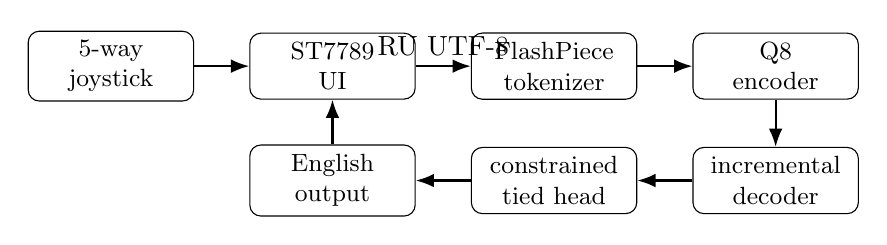
\begin{tikzpicture}[
node distance=6mm and 7mm,
box/.style={draw,rounded corners,align=center,minimum height=8mm,minimum width=21mm,font=\small},
arr/.style={-Latex,thick}]
\node[box] (joy) {5-way\\joystick};
\node[box,right=of joy] (ui) {ST7789\\UI};
\node[box,right=of ui] (tok) {FlashPiece\\tokenizer};
\node[box,right=of tok] (enc) {Q8\\encoder};
\node[box,below=of enc] (dec) {incremental\\decoder};
\node[box,left=of dec] (head) {constrained\\tied head};
\node[box,left=of head] (out) {English\\output};
\draw[arr] (joy)--(ui);
\draw[arr] (ui)--node[above]{RU UTF-8}(tok);
\draw[arr] (tok)--(enc);
\draw[arr] (enc)--(dec);
\draw[arr] (dec)--(head);
\draw[arr] (head)--(out);
\draw[arr] (out)--(ui);
\end{tikzpicture}
\caption{End-to-end offline translation path.}
\label{fig:path}
\end{figure}

\section{Related work}
The student architecture follows the encoder--decoder Transformer family \citep{vaswani2017attention}. Subword NMT showed the importance of subword units for open-vocabulary translation \citep{sennrich2016subword}; FlashPiece adapts this principle to a microcontroller by guaranteeing coverage with all 256 byte values and using a minimal greedy decoder.

Sequence-level knowledge distillation simplifies a student's target distribution by replacing ambiguous human targets with teacher translations \citep{kim2016sequence}. This is especially attractive for a model near one million parameters. Tied input/output embeddings reduce storage and have been shown to be effective in language models \citep{press2017using}. RMSNorm reduces normalization overhead by removing explicit mean centering \citep{zhang2019rmsnorm}.

Integer quantization is a standard technique for efficient inference \citep{jacob2018quantization}. Prior NMT work has also demonstrated that carefully trained low-bit translation models can reach 4-bit precision \citep{aji2019fourbit}, motivating our Q4 roadmap. We do not, however, label the Q4 path as implemented.

Connectionist-temporal-classification non-autoregressive translation can eliminate token-by-token decoder dependencies \citep{libovicky2018ctc}. Yet realistic evaluation has shown that NAR is not automatically faster than an optimized autoregressive system, especially when wall-clock latency and small batches are considered \citep{helcl2022nar}. Our deployment batch size is exactly one, so the default path is autoregressive and CTC remains experimental.

On microcontrollers, MCUNet established the value of model/runtime co-design \citep{lin2020mcunet}. ESP32-S3 community runtimes demonstrate that transformer-like dense workloads can use PIE signed-int8 vector operations effectively \citep{dory2026esp32llm,bareiro2026commands}. \modelname applies these ideas to sequence-to-sequence translation rather than language-model completion or command parsing.

\section{Problem formulation}
Let normalized Russian input be represented by
\begin{equation}
\mathbf{x}=(x_1,\dots,x_S),\qquad S\le S_{\max}=64,
\end{equation}
and an English target by
\begin{equation}
\mathbf{y}=(y_1,\dots,y_T),\qquad T\le T_{\max}=48.
\end{equation}
The autoregressive model defines
\begin{equation}
p_\theta(\mathbf{y}\mid\mathbf{x})
=\prod_{t=1}^{T}p_\theta(y_t\mid y_{<t},\mathbf{x}).
\end{equation}

Deployment is multi-objective. For architecture $a$ and numeric format $q$:
\begin{align}
\min_{a,q}\quad
&\mathcal{L}_{MT}(a,q)+\lambda_L L_1(a,q)+\lambda_M M(a,q),\\
\text{s.t.}\quad
&B_{\mathrm{flash}}\le 16\text{ MB},\\
&B_{\mathrm{PSRAM}}\le 8\text{ MB},\\
&B_{\mathrm{hot}}\le B_{\mathrm{internal}},\\
&S\le 64,\quad T\le48.
\end{align}
$L_1$ denotes batch-one wall-clock latency. We do not assign arbitrary weights to these terms; instead we derive dominant storage/compute terms and then define a physical benchmark protocol.

\section{FlashPiece tokenizer}
\subsection{Lossless byte foundation}
FlashPiece operates on normalized UTF-8 bytes. IDs 0--3 are PAD, BOS, EOS, and UNK. The next 256 IDs represent every possible byte. Thus any UTF-8 input is representable even if no learned multi-byte piece matches.

Additional pieces are frequent byte n-grams from the distilled training corpus. For candidate piece $p$ with byte length $|p|$ and frequency $f(p)$, the current builder ranks by approximate byte savings
\begin{equation}
\operatorname{score}(p)=f(p)(|p|-1).
\end{equation}
The vocabulary is built only from training data. Validation and test references never influence token selection.

\subsection{Greedy encoding}
At byte position $i$, the encoder searches only pieces beginning with $b_i$ and selects the longest match:
\begin{equation}
p^\star=\arg\max_{p\in\mathcal{V}_{b_i}} |p|
\quad\text{s.t.}\quad b_{i:i+|p|-1}=p.
\end{equation}
The C++ runtime precomputes 256 first-byte buckets once at model load. This changes input tokenization from a vocabulary-wide scan at every byte to a small bucket search.

\subsection{Vocabulary as a hardware parameter}
A larger vocabulary can reduce source and target sequence lengths, but it also increases output-head work. If the decoder scores $C$ allowed candidates at each of $T$ generated steps with width $d$, the tied output head requires
\begin{equation}
M_{\mathrm{head}}=TCd
\label{eq:head}
\end{equation}
dot-product MACs. Thus vocabulary size is simultaneously an NLP and systems variable.

\section{Student Transformer}
The default configuration is
\begin{equation}
(V,d,f,H,L_e,L_d,S_{\max},T_{\max})
=(1536,128,256,4,3,2,64,48).
\end{equation}
All dense layers are bias-free. Source and target positions use separate learned embeddings.

\subsection{RMSNorm and residual structure}
For hidden vector $\mathbf{h}\in\R^d$ and learned gain $\mathbf{g}$:
\begin{equation}
\rms(\mathbf{h})
=\mathbf{g}\odot
\frac{\mathbf{h}}
{\sqrt{d^{-1}\sum_{i=1}^{d}h_i^2+\epsilon}},
\qquad\epsilon=10^{-5}.
\end{equation}
An encoder block is
\begin{align}
\mathbf{u}&=\mathbf{h}+
\mathrm{MHA}(\rms(\mathbf{h})),\\
\mathbf{h}'&=\mathbf{u}+
W_2\silu(W_1\rms(\mathbf{u})).
\end{align}
A decoder block adds causal self-attention and cross-attention:
\begin{align}
\mathbf{u}&=\mathbf{h}+
\mathrm{MHA}_{self}(\rms(\mathbf{h})),\\
\mathbf{v}&=\mathbf{u}+
\mathrm{MHA}_{cross}(\rms(\mathbf{u}),\mathbf{H}_e),\\
\mathbf{h}'&=\mathbf{v}+
W_2\silu(W_1\rms(\mathbf{v})).
\end{align}

\subsection{Attention}
For a head width $d_h=d/H$,
\begin{equation}
\mathrm{Attn}(Q,K,V)
=\softmax\left(\frac{QK^\top}{\sqrt{d_h}}+M\right)V,
\end{equation}
where $M$ is the causal mask for decoder self-attention.

\subsection{Tied and constrained output head}
Let $E\in\R^{V\times d}$ be the token embedding matrix. The output classifier reuses $E$:
\begin{equation}
\ell_t(j)=\frac{E_j^\top h_t}{\sqrt{d}}.
\end{equation}
Because deployment is strictly Russian-to-English, the runtime precomputes
\begin{equation}
\mathcal{C}
=\{\mathrm{EOS}\}\cup
\{j:\operatorname{bytes}(j)\subseteq[0x20,0x7E]\}.
\end{equation}
Only IDs in $\mathcal{C}$ are scored at inference. This is not algebraically equivalent to full-vocabulary decoding: if a removed source-language token would otherwise win, the output changes. We therefore describe this correctly as constrained decoding. Training targets are normalized to printable ASCII, and evaluation preserves raw references so the deployment normalization penalty can be measured.

\section{Training and distillation}
\subsection{Data}
The recommended starting corpus is OPUS-100 \citep{zhang2020opus100,hf_opus100}. The downloader preserves the dataset's train/validation/test separation, creates a device-normalized English view, and separately saves raw validation and test English references.

\subsection{Sequence-level teacher targets}
For teacher distribution $q_\phi$:
\begin{equation}
\hat{\mathbf{y}}
=\arg\max_{\mathbf{y}}q_\phi(\mathbf{y}\mid\mathbf{x}),
\end{equation}
approximated by beam search. The student minimizes
\begin{equation}
\mathcal{L}_{KD}
=-\sum_t\log p_\theta(
\hat y_t\mid\hat y_{<t},\mathbf{x}).
\end{equation}
The reference implementation uses \texttt{Helsinki-NLP/opus-mt-ru-en} as a workstation-side teacher. The teacher never runs on ESP32.

An important pipeline detail is ordering: FlashPiece is built after distillation on Russian source plus teacher English. With a fixed vocabulary budget, this allocates pieces to the exact target distribution seen by the student rather than to unused human-reference variants.

\section{Row-wise Q8 inference}
\subsection{Weight quantization}
For row $\mathbf{w}_r\in\R^n$:
\begin{align}
s_r&=\frac{\max_j|w_{rj}|}{127},\\
q_{rj}&=\operatorname{clip}
\left(\operatorname{round}(w_{rj}/s_r),-127,127\right).
\end{align}
Each row stores one FP32 scale and $n$ signed bytes. A zero row receives scale one.

For activation vector $\mathbf{x}$:
\begin{align}
s_x&=\frac{\max_j|x_j|}{127},\\
q^x_j&=\operatorname{clip}
\left(\operatorname{round}(x_j/s_x),-127,127\right).
\end{align}
The reconstructed matvec is
\begin{equation}
\hat y_r=s_rs_x\sum_{j=1}^{n}q_{rj}q^x_j.
\label{eq:q8}
\end{equation}
The inner sum accumulates into INT32.

\subsection{Rounding-error expression}
Write
\begin{align}
w_j&=s_rq^w_j+\delta w_j,\\
x_j&=s_xq^x_j+\delta x_j,
\end{align}
with $|\delta w_j|\le s_r/2$ and $|\delta x_j|\le s_x/2$ under nearest rounding. Then
\begin{align}
w^\top x-\hat y
=\sum_j(
s_rq^w_j\delta x_j
+s_xq^x_j\delta w_j
+\delta w_j\delta x_j).
\end{align}
A conservative bound is
\begin{equation}
|e|\le
\frac{s_x}{2}\sum_j|s_rq^w_j|
+\frac{s_r}{2}\sum_j|s_xq^x_j|
+\frac{ns_rs_x}{4}.
\end{equation}
This is not a quality guarantee; it motivates later calibration and QAT experiments.

\subsection{Why Q8 first}
ESP-DL currently presents W8A8 as the fastest general quantized deployment mode \citep{espressif_espdl}, and ESP-NN contains S3-specific int8 kernels \citep{espressif_espnn}. Q8 therefore provides a simple, verifiable baseline. Q4 is attractive because it reduces weight traffic, and prior NMT work indicates low-bit translation is plausible \citep{aji2019fourbit}, but Q4 only improves latency if reduced memory traffic outweighs unpacking overhead. We treat Q4 as a hypothesis until benchmarked.

\section{Model binary format}
The exporter produces a single memory-mappable \texttt{.s3mt} file. The fixed 128-byte little-endian header stores magic, version, architecture dimensions, special token IDs, tokenizer bytes, payload bytes, CRC32, and total length. Tokenizer pieces are followed by tensors in fixed architecture order. Matrix rows and scale blocks are 16-byte aligned.

\begin{figure}[t]
\centering
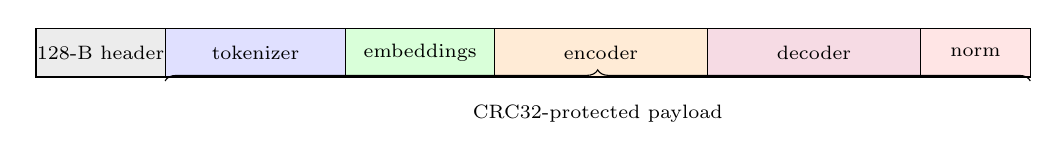
\begin{tikzpicture}[x=.82cm,y=.62cm,font=\scriptsize]
\draw[fill=gray!15] (0,0) rectangle (2,1);
\node at (1,.5){128-B header};
\draw[fill=blue!12] (2,0) rectangle (4.8,1);
\node at (3.4,.5){tokenizer};
\draw[fill=green!15] (4.8,0) rectangle (7.1,1);
\node at (5.95,.5){embeddings};
\draw[fill=orange!16] (7.1,0) rectangle (10.4,1);
\node at (8.75,.5){encoder};
\draw[fill=purple!14] (10.4,0) rectangle (13.7,1);
\node at (12.05,.5){decoder};
\draw[fill=red!10] (13.7,0) rectangle (15.4,1);
\node at (14.55,.5){norm};
\draw[decorate,decoration={brace,amplitude=4pt}]
(2,-.08)--(15.4,-.08)
node[midway,below=5pt]{CRC32-protected payload};
\end{tikzpicture}
\caption{Logical \texttt{.s3mt} layout.}
\end{figure}

Before exposing tensor pointers, the C++ loader checks CRC32, total/payload/tokenizer lengths, vocabulary bounds, hidden-width alignment, FFN bounds, head divisibility, layer counts, sequence limits, special token IDs, every tensor shape, and absence of trailing data. Corruption becomes a deterministic load error instead of undefined memory access.

\section{Portable runtime and ESP32-S3 specialization}
\subsection{Parity-first implementation}
The exact same C++ model parser, tokenizer, encoder, decoder, and output projection are compiled for a host CLI and the ESP-IDF firmware. This allows exporter/runtime bugs to be reproduced without a flash cycle.

\subsection{PIE int8 dot product}
The ESP32-S3 path uses aligned 128-bit vector loads and signed int8 multiply-accumulate operations. Conceptually:
\begin{equation}
a=\sum_{j=1}^{n}q^x_jq^w_j.
\end{equation}
The runtime processes 16 signed bytes per vector step and retains a scalar fallback. The approach follows the same class of S3 optimization used in ESP-NN and public S3 transformer runtimes \citep{espressif_espnn,dory2026esp32llm}.

\subsection{Incremental decoder}
For decoder layer $\ell$, the runtime stores self-attention
\begin{equation}
K^{(\ell)}_{1:t},V^{(\ell)}_{1:t}
\end{equation}
so previous token projections are never recomputed. Cross-attention keys and values for the source sequence are computed once before autoregressive generation. Only the current token's self Q/K/V, cross Q, output projections, FFN, and tied output head are evaluated at each step.

\section{Exact analytical budgets}
\subsection{Parameter formula}
For vocabulary $V$, width $d$, FFN width $f$, encoder depth $L_e$, decoder depth $L_d$, and maximum source/target lengths $S_m,T_m$:
\begin{align}
P={}&Vd+(S_m+T_m)d\\
&+L_e(4d^2+2df)\\
&+L_d(8d^2+2df)\\
&+(2L_e+3L_d+1)d.
\label{eq:param}
\end{align}
For the base preset:
\begin{align}
P_{tok}&=1536(128)=196{,}608,\\
P_{pos}&=(64+48)(128)=14{,}336,\\
P_{enc}&=3(4(128)^2+2(128)(256))=393{,}216,\\
P_{dec}&=2(8(128)^2+2(128)(256))=393{,}216,\\
P_{norm}&=(2(3)+3(2)+1)(128)=1{,}664,
\end{align}
hence
\begin{equation}
P=999{,}040.
\end{equation}

\subsection{Serialized Q8 storage}
All non-norm learned values are quantized:
\begin{equation}
Q=P-P_{norm}=997{,}376.
\end{equation}
The exact number of row scales is
\begin{align}
R={}&V+S_m+T_m\\
&+L_e(5d+f)+L_d(9d+f)\\
={}&7{,}152.
\end{align}
Ignoring small tensor headers, tokenizer strings, and alignment padding:
\begin{equation}
B_{Q8}=Q+4R+4P_{norm}
=1{,}032{,}640\text{ bytes}
=1008.44\text{ KiB}.
\end{equation}
A derived packed-Q4 estimate retaining FP32 scales and norms is
\begin{equation}
B_{Q4}^{est}
=\left\lceil Q/2\right\rceil+4R+4P_{norm}
=533{,}952\text{ bytes}
=521.44\text{ KiB}.
\end{equation}
No Q4 speed claim is made.

\begin{table}[t]
\centering
\caption{Exact preset budgets at vocabulary 1,536. Q4 is a storage estimate only.}
\begin{tabular}{lrrrrr}
\toprule
Preset & $d$ & $L_e/L_d$ & Params & Q8 KiB & Q4 est. KiB\\
\midrule
Tiny & 96 & 2/2 & 527,904 & 538.6 & 281.3\\
Base & 128 & 3/2 & 999,040 & 1008.4 & 521.4\\
Quality & 160 & 4/2 & 1,699,680 & 1704.6 & 875.8\\
\bottomrule
\end{tabular}
\end{table}

\subsection{Mutable memory}
The maximum FP32 encoder state is
\begin{equation}
B_{enc}=S_md(4),
\end{equation}
which is 32 KiB for base. Current FP32 decoder self/cross caches consume
\begin{equation}
B_{cache}
=L_d[2T_md+2S_md](4)
=229{,}376\text{ bytes}
=224\text{ KiB}.
\end{equation}
The RGB565 240$\times$240 framebuffer uses 115,200 bytes (112.5 KiB), and the 20-row DMA strip uses 9,600 bytes (9.375 KiB).

\subsection{Dense MAC model}
For source length $S$:
\begin{equation}
M_e=L_e(4Sd^2+2S^2d+2Sdf).
\end{equation}
Cross-attention K/V precompute:
\begin{equation}
M_{xKV}=L_d(2Sd^2).
\end{equation}
At decoder step $t$:
\begin{equation}
M_{d,t}
=L_d(6d^2+2df+2d(t+S)).
\end{equation}
The output head is Eq.~\ref{eq:head}. At representative $S=32,T=24,C=1536$, the exact analytical script gives:
\begin{align}
M_e&=13.369344\text{ M},\\
M_{xKV}&=2.097152\text{ M},\\
M_{decoder}&=8.411136\text{ M},\\
M_{head}&=4.718592\text{ M},\\
M_{total}&=28.596224\text{ M MACs}.
\end{align}
The output head alone contributes about 16.5\% of these dense MACs and also repeatedly streams embedding rows, making candidate pruning attractive.

\begin{figure}[t]
\centering
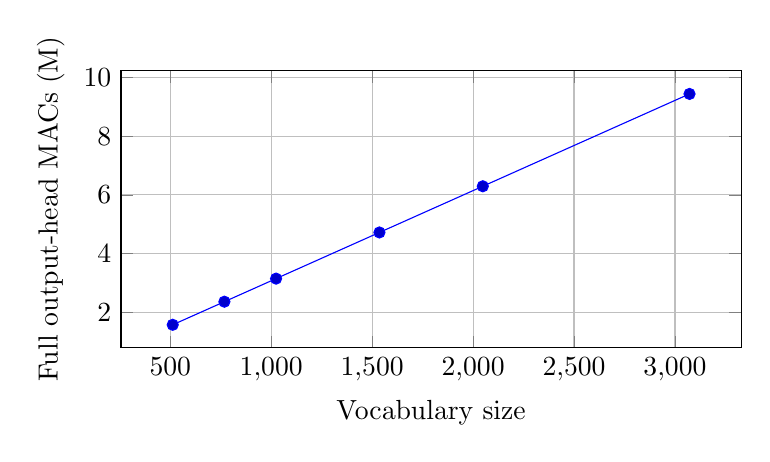
\begin{tikzpicture}
\begin{axis}[
width=.78\linewidth,height=5.1cm,
xlabel={Vocabulary size},
ylabel={Full output-head MACs (M)},
grid=major]
\addplot+[mark=*] coordinates {
(512,1.572864)
(768,2.359296)
(1024,3.145728)
(1536,4.718592)
(2048,6.291456)
(3072,9.437184)};
\end{axis}
\end{tikzpicture}
\caption{Output projection cost for $T=24,d=128$ when every vocabulary row is scored. The deployed constrained head scores only English-compatible IDs.}
\end{figure}

\subsection{Roofline-style interpretation}
A useful lower-bound model is
\begin{equation}
L\gtrsim
\max\left(
\frac{M}{\Pi_{\mathrm{MAC}}},
\frac{B_{\mathrm{read}}}{\beta_{\mathrm{mem}}}
\right)
+L_{\mathrm{softmax}}+L_{\mathrm{control}}.
\end{equation}
$\Pi_{\mathrm{MAC}}$ and $\beta_{\mathrm{mem}}$ must be measured on the actual board; host values are not substituted. This model explains why Q4 may help a bandwidth-bound configuration and why a second core may not help if both cores contend for the same external-memory path.

\section{Physical interface}
The firmware renders a six-row Russian keyboard and input/output text on a 240$\times$240 ST7789. A five-way active-low joystick uses internal pull-ups. Example configurable pins are shown below.

\begin{table}[H]
\centering
\begin{tabular}{lll}
\toprule
Signal & Default GPIO & Direction\\
\midrule
LCD MOSI & 11 & MCU$\rightarrow$LCD\\
LCD SCLK & 12 & MCU$\rightarrow$LCD\\
LCD CS/DC/RST/BL & 10/9/8/7 & MCU$\rightarrow$LCD\\
Joystick U/D/L/R & 4/5/6/13 & input\\
Joystick press & 14 & input\\
\bottomrule
\end{tabular}
\end{table}
These pins are examples, not universal board wiring. Development-board schematics must be checked before use.

The framebuffer is allocated in PSRAM. A 20-row DMA-capable strip lives in internal RAM. ESP-IDF LCD transfers are asynchronous, so the code waits for the color-transfer-complete callback before overwriting that strip. This avoids a subtle corruption mode in which the CPU reuses a buffer while SPI DMA still owns it.

\section{Measured correctness experiment}
\subsection{Evidence categories}
We separate:
\begin{enumerate}[leftmargin=*]
\item \textbf{Measured}: host compilation, tokenizer tests, toy training, Q8 export, C++ parity, CRC rejection;
\item \textbf{Exact analytical}: parameter count, Q8 bytes, cache bytes, framebuffer bytes, dense MACs;
\item \textbf{Derived estimate}: packed-Q4 model bytes;
\item \textbf{Unverified}: held-out full-model BLEU/chrF/COMET, physical ESP32 latency, tokens/s, energy, thermal behavior.
\end{enumerate}

\subsection{Toy memorization and Q8 parity}
A deterministic script uses 20 small RU--EN pairs, a 320-entry FlashPiece tokenizer, one encoder layer, one decoder layer, $d=32$, $f=64$, four heads, and seed 0. It trains for 600 steps and records loss every ten updates. The measured cross-entropy decreases from
\begin{equation}
5.7639008\rightarrow0.04127665.
\end{equation}
PyTorch greedy decoding exactly reproduces 20/20 training targets. The exported row-wise-Q8 model loaded by the portable C++ runtime also exactly reproduces 20/20 training targets. The Russian greeting used in the smoke set maps to \texttt{hello}. A deliberately flipped payload byte causes the C++ loader to fail with a CRC32 mismatch.

This test demonstrates end-to-end implementation parity. It is intentionally \emph{not} a held-out NMT benchmark.

\begin{figure}[t]
\centering
\begin{tikzpicture}
\begin{axis}[
width=.80\linewidth,height=5.2cm,
xlabel={Training step},
ylabel={Cross-entropy},
ymode=log,
grid=major]
\addplot+[mark=none,thick]
table[x=step,y=cross_entropy,col sep=comma]
{data/smoke_loss.csv};
\end{axis}
\end{tikzpicture}
\caption{Measured toy memorization loss, recorded every ten steps by the reproducibility script.}
\end{figure}

\begin{table}[t]
\centering
\caption{Current verification status.}
\begin{tabular}{ll}
\toprule
Check & Result\\
\midrule
FlashPiece unit tests & pass\\
Host C++ build & pass\\
PyTorch toy train exact & 20/20\\
Q8 C++ toy train exact & 20/20\\
Loss & 5.7639 $\rightarrow$ 0.04128\\
Corrupt model & rejected by CRC\\
Physical ESP32 BLEU/latency & not yet measured\\
\bottomrule
\end{tabular}
\end{table}

\section{Full evaluation protocol}
\subsection{Translation quality}
Final checkpoints should be evaluated on the frozen OPUS-100 test split. BLEU should be produced through SacreBLEU to avoid hidden preprocessing differences \citep{post2018sacrebleu}. We also report chrF \citep{popovic2015chrf}. COMET \citep{rei2020comet} can be computed offline on a workstation. Metrics should be calculated both against the device-normalized English view and the preserved raw English references.

\subsection{Architecture sweep}
A controlled sweep should hold teacher, train split, random seeds, optimizer, and test set fixed:
\begin{table}[H]
\centering
\begin{tabular}{lrrrrl}
\toprule
Run & $V$ & $d$ & $L_e/L_d$ & $f$ & Goal\\
\midrule
T1 & 768 & 96 & 2/2 & 192 & speed floor\\
B1 & 1024 & 128 & 3/2 & 256 & vocab tradeoff\\
B2 & 1536 & 128 & 3/2 & 256 & default\\
B3 & 2048 & 128 & 3/2 & 256 & shorter sequences\\
Q1 & 1536 & 160 & 4/2 & 320 & quality ceiling\\
\bottomrule
\end{tabular}
\end{table}

\subsection{Physical-board benchmark}
For every exported model:
\begin{enumerate}[leftmargin=*]
\item use the same N16R8 board, CPU clock, flash mode, PSRAM mode, compiler flags, and firmware commit;
\item warm up with at least five translations;
\item measure a fixed battery of short, medium, and long sentences;
\item record source tokens, output tokens, encoder microseconds, decoder microseconds, total latency, and tokens/s;
\item record internal-RAM and PSRAM free/low-water marks;
\item repeat each sentence at least 30 times;
\item report median and interquartile range rather than minimum latency;
\item save model checksum, ESP-IDF version, chip revision, and firmware Git SHA.
\end{enumerate}

\begin{table}[H]
\centering
\caption{Physical-board results intentionally blank until measurements exist.}
\begin{tabular}{lrrrrrr}
\toprule
Model & BLEU & chrF & Enc ms & Dec ms & Total ms & tok/s\\
\midrule
Tiny Q8 & -- & -- & -- & -- & -- & --\\
Base Q8 & -- & -- & -- & -- & -- & --\\
Base Q4 & -- & -- & -- & -- & -- & --\\
CTC/NAR & -- & -- & -- & -- & -- & --\\
\bottomrule
\end{tabular}
\end{table}

\section{Optimization roadmap}
\subsection{Vocabulary sweep before scaling width}
Equation~\ref{eq:head} shows that vocabulary directly controls repeated decoder cost. Smaller vocabularies lengthen sequences; larger vocabularies increase classifier traffic. The optimum must be measured rather than assumed.

\subsection{Packed Q4}
The exact base Q8 tensor payload is 1008.44 KiB; the packed-Q4 estimate is 521.44 KiB. If inference is bandwidth-limited, this may be the largest remaining speed lever. If nibble extraction dominates, Q4 can lose. A custom PIE Q4$\times$Q8 kernel should therefore be benchmarked against Q8 on identical checkpoints.

\subsection{Quantized decoder caches}
The current FP32 decoder cache is 224 KiB. INT8 cache storage could reduce raw cache value bytes by roughly four times before adding scales. The quality impact of per-vector versus per-head scales should be measured.

\subsection{Fusion}
RMSNorm, activation quantization, and projection currently form separate logical passes. A fused path can compute norm statistics, emit an aligned Q8 activation vector, and immediately perform the matvec, reducing hot-vector memory traffic.

\subsection{Dual-core execution}
A second LX7 core only helps if the kernel is compute-bound. If model rows already saturate flash/PSRAM/cache bandwidth, dividing rows across two cores can add contention. This must be established by profiling, consistent with bandwidth limits observed in other ESP32-S3 Transformer experiments \citep{dory2026esp32llm}.

\subsection{CTC/NAR}
The repository contains an experimental CTC-style encoder path. Its acceptance criterion is batch-one wall-clock latency on the actual S3 at acceptable BLEU/chrF. GPU throughput is irrelevant to this product. This conservative criterion follows the warning that NAR systems are not always as fast as headline parallelism suggests under realistic evaluation \citep{helcl2022nar}.

\section{Limitations}
The current empirical result proves pipeline correctness, not general translation quality. No full-data model has yet been reported here with held-out BLEU/chrF. The physical firmware still needs measurement on the user's exact board/display assembly. The output constraint normalizes English to printable ASCII, so diacritics and typography can be lost. Q8 is post-training export rather than a full quantization-aware training study. Analytical MAC counts exclude softmax exponentials, normalization, tokenization, cache misses, control overhead, and display I/O, so they must not be presented as latency predictions. OPUS-100 is heterogeneous and may not match every real domain. Q4, quantized caches, dual-core execution, and NAR remain hypotheses until benchmarked.

\section{Conclusion}
\modelname treats translation on an ESP32-S3 as a hardware--software co-design problem rather than a demonstration of fitting the largest possible language model. A scoped RU$\rightarrow$EN system can combine a roughly one-million-parameter Transformer, a 1.5k lossless byte-piece vocabulary, teacher distillation, tied embeddings, row-wise Q8 weights, incremental decoding, constrained output scoring, a memory-mappable binary, and a low-memory physical UI. The complete PyTorch$\rightarrow$Q8$\rightarrow$C++ path is already verified by a deterministic parity test, and all central memory/compute quantities are derived exactly. The next scientific step is to train the full distilled grid and populate the deliberately blank physical-board quality/latency table.

\section*{Reproducibility}
The repository contains the tokenizer, PyTorch architecture, OPUS-100 downloader, teacher distillation script, trainer, evaluator, Q8 exporter, model checker, analytical scripts, portable C++ runtime, ESP-IDF firmware, host CLI, tests, and CI. A typical workflow is:

\begin{verbatim}
python scripts/download_opus100.py --out-dir data/opus100 --limit-train 500000
python model/distill_teacher.py --input data/opus100/train.tsv \
  --output data/distilled.tsv
python model/tokenizer.py build --input data/distilled.tsv \
  --output artifacts/tokenizer.json --vocab-size 1536
python model/train.py --train data/distilled.tsv \
  --val data/opus100/validation.tsv \
  --tokenizer artifacts/tokenizer.json --preset base --out artifacts/base
python model/evaluate.py --checkpoint artifacts/base/best.pt \
  --tokenizer artifacts/tokenizer.json --data data/opus100/test.tsv \
  --raw-data data/opus100/test.raw.tsv
python model/export_s3mt.py --checkpoint artifacts/base/best.pt \
  --tokenizer artifacts/tokenizer.json --output artifacts/nanotranslate.s3mt
cmake -S host -B host/build
cmake --build host/build -j
./host/build/nanomt_cli artifacts/nanotranslate.s3mt
\end{verbatim}

\begin{ack}
This is an independent student engineering research project. Open academic literature, Espressif documentation, and public reference runtimes informed the design. No physical-device performance numbers are claimed without measurement.
\end{ack}

\bibliographystyle{plainnat}
\bibliography{refs}

\appendix
\section{Binary header schema}
The fixed \texttt{.s3mt} header is 128 bytes, little-endian. Its fields are:
\begin{table}[H]
\centering
\begin{tabular}{rll}
\toprule
Offset & Type & Meaning\\
\midrule
0 & char[8] & magic \texttt{S3MT0001}\\
8 & u32 & format version\\
12 & u32 & flags\\
16--52 & u32 & vocab, $d$, $f$, heads, layers, max lengths\\
56--68 & u32 & PAD/BOS/EOS/UNK IDs\\
64 & u32 & tokenizer payload bytes\\
68 & u32 & protected payload bytes\\
72 & u32 & CRC32 over payload\\
76 & u32 & total file bytes\\
80--127 & reserved & zero/future fields\\
\bottomrule
\end{tabular}
\end{table}
A Q8 tensor stores a small shape header, one FP32 scale per output row, alignment padding, signed-int8 row-major values, then trailing alignment. RMSNorm vectors remain FP32.

\section{Base parameter derivation}
For base:
\begin{align}
P_{tok}&=1536(128)=196{,}608,\\
P_{pos}&=(64+48)(128)=14{,}336,\\
P_{enc}&=3[4(128)^2+2(128)(256)]=393{,}216,\\
P_{dec}&=2[8(128)^2+2(128)(256)]=393{,}216,\\
P_{norm}&=13(128)=1{,}664.
\end{align}
Their sum is exactly 999,040.

\section{Default wiring}
The firmware defaults to ST7789 MOSI/SCLK/CS/DC/RST/BL on GPIO 11/12/10/9/8/7 and joystick up/down/left/right/press on GPIO 4/5/6/13/14. All are configurable in \texttt{menuconfig}. These are logical defaults, not a universal electrical schematic. The user's development board and display module documentation must determine available GPIOs and supply wiring.

\section{Checklist before publishing ESP32 measurements}
Every physical result should record board/module part number, chip revision, ESP-IDF version, compiler version, CPU clock, flash mode/frequency, PSRAM mode/frequency, model checksum, firmware commit, sentence battery, warm-up count, repetition count, latency median/IQR, and memory low-water marks. This prevents a single optimistic timing from becoming an irreproducible performance claim.

\end{document}
